\chapter{ユーザインタフェース}
\label{chap:userinterface}
文字入力を行うほとんどのユーザーはIMEを利用する際にアプリケーションごとに
IMEを変えたりせず、
あらゆるアプリケーションに対して同じIMEを利用する。
そこで基本的な入力をすることができ、
かつ推薦機構の導入を実現しなければならない。
そこでIME本来の機能を損なわないように
Rive Clientに
独自のインタフェースを実装することでRive日本語入力システムを実現した。
またこれらのユーザインタフェースは日本語独自の
設計ではないため容易に外国語のIMEへの実装が可能である。

\newpage
\section{キーボード}
モバイルデバイス使用者が使う入力のうち最も使用者が多い二つの
キーボードを使用可能にした。
キーボードはqwertyキーボードとフリック入力キーボードの二つを実装した。
ユーザーは好みに合わせて二つのキーボードを使用することができる。
(実装したキーボード図:\ref{fig:qwerty},図:\ref{fig:flick})
\begin{figure}[htbp]
  \begin{minipage}{0.5\hsize}
    \begin{center}
      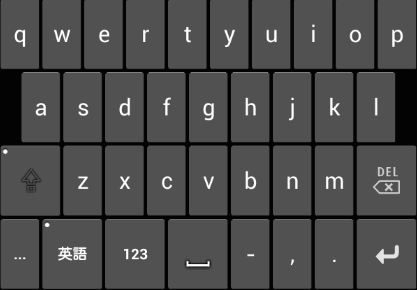
\includegraphics[width=7cm,bb=0 0 417 290]{images/qwerty.png}
    \end{center}
    \caption{qwertyキーボード}
    \label{fig:qwerty}
  \end{minipage}
  \begin{minipage}{0.5\hsize}
    \begin{center}
      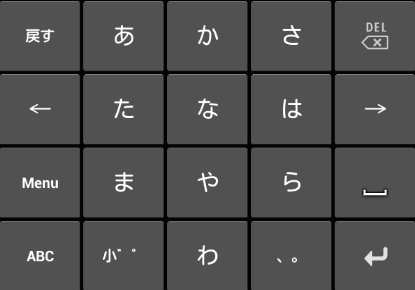
\includegraphics[width=7cm,bb=0 0 415 290]{images/flick.png}
    \end{center}
    \caption{flickキーボード}
    \label{fig:flick}
  \end{minipage}
\end{figure}

\section{ダブル辞書インタフェース}
IMEとしての通常の文字変換もないと普段の使用に耐えることができないため、
二つの変換システムを実装している。
上段はコンテキストによる推薦システム\ref{chap:recommend}から推薦される候補単語で、
下段は通常のIMEに搭載されている辞書である。
それぞれ横方向にスクロールさせることで候補を見ていくことができる。
(ダブル辞書インタフェース画面:\ref{fig:doubledic})
\begin{figure}[htbp]
  \begin{center}
    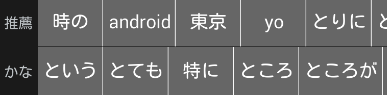
\includegraphics[width=120mm,bb=0 0 387 95]{images/doubledic.png}
  \end{center}
  \label{fig:doubledic}
  \caption{ダブル辞書インタフェース画面}
\end{figure}

\section{単語変換機能}
\label{wordflick}
この機能は候補単語をフリック操作することで、
フリックした候補単語を元に、新たな候補単語郡を推薦する。
現在上方向へのフリック操作では英語変換をし、
下方向へのフリック操作では類語変換を行う。
この機能があることによって推薦単語が無意味になる可能性を減らすと共に、
入力の多様性を確保する。
この単語変換機能は上下段両方に使用可能な機能である。
この機能は連続で使用することができるため、
類語から類語へと連続で新しい候補を辿ることや、
類語変換したものを英語へ変換するといったことが可能である。
(単語フリックイメージ図:\ref{fig:wordflick})
\begin{figure}[htbp]
  \begin{center}
    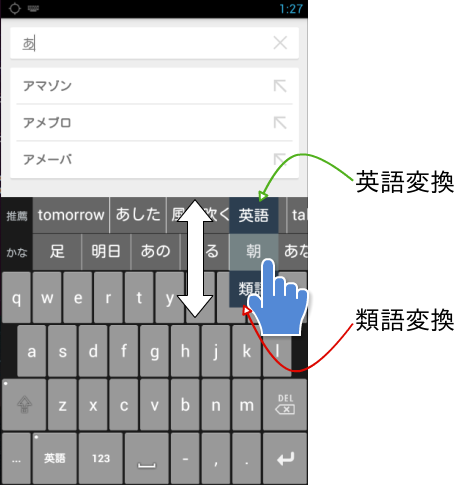
\includegraphics[width=14cm,bb=0 0 461 485]{images/candidateflick.png}
  \end{center}
  \caption{単語フリックイメージ図}
  \label{fig:wordflick}
\end{figure}

\section{候補ビューの横スクロール}
上下段どちらかの候補ビューを横にスクロールする際に、
もう一方も連動して動かせるように実装した。
候補ビューをスクロールさせる際にはどちらの段にも表示されていない単語を
入力したい場合なので、
共にスクロールすることで入力したい単語の検索を助ける。
スクロールする方向はもう一方の段のスクロールに対し、
順方向と逆方向の二通りから選択可能である。

